\documentclass[tikz,border=10pt]{standalone}
% no extra libraries needed
\begin{document}
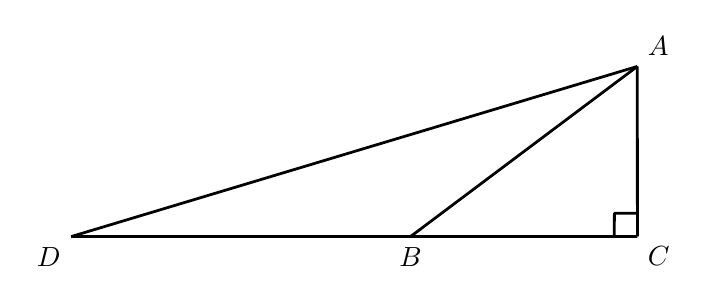
\begin{tikzpicture}[line width=1.0pt, line join=round, font=\fontsize{10}{12}\selectfont]
  % Named points (converted from pixel coords, s = 0.012214 cm/px)
  \coordinate (D) at (-3.5539997310861695,-1.0820155217812877);
  \coordinate (B) at (0.7569999666224292,-1.0808739534894622);
  \coordinate (C) at (3.6367857525902028,-1.0801113758111902);
  \coordinate (A) at (3.636214011873537,1.0790008510819402);

  % Right-angle marker at C (one square, 24 px side)
  \coordinate (R1) at (3.3437857628629217,-1.0801889632668227);
  \coordinate (R2) at (3.3446577120036087,-0.7871871835011268);
  \coordinate (R3) at (3.6376577017308898,-0.7871095960454942);

  % Segments
  \draw (A) -- (D);      % long slanted line
  \draw (D) -- (C);      % horizontal baseline through B
  \draw (A) -- (C);      % vertical right side
  \draw (A) -- (B);      % slanted segment

  % Right-angle mark (single)
  \draw (R1) -- (R2) -- (R3);

  % Labels
  \node[above right] at (A) {$A$};
  \node[below left]  at (D) {$D$};
  \node[below]       at (B) {$B$};
  \node[below right] at (C) {$C$};
\end{tikzpicture}
\end{document}